\documentclass{article}
\usepackage{amsmath}
\usepackage{parskip}
\usepackage{tikz}

\begin{document}
A simple pendulum consists of a string of length $\ell$ attached to the origin and an object with position $(x, y)$. The object's angular displacement is $\theta$. This situation is visualized in the diagram below.

\begin{figure}[h]
  \centering
  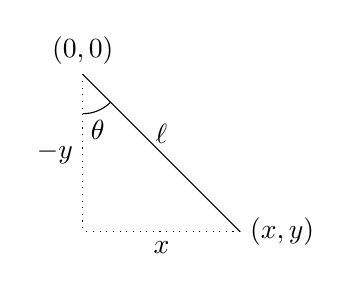
\begin{tikzpicture}
    \coordinate (origin)    at (0, 0);
    \coordinate (object)    at (2, -2);
    \coordinate (imaginary) at (0, -2);

    \node[above] at (origin) {$(0,0)$};
    \node[right] at (object) {$(x,y)$};

    \draw (origin) -- (object) node[above,pos=0.5]{$\ell$};
    \draw[dotted] (object) -- (imaginary) node[pos=0.5,below]{$x$};
    \draw[dotted] (origin) -- (imaginary) node[pos=0.5,left]{$-y$};
    \draw (0, -0.5)  arc[radius = 0.5, start angle= -90, end angle= -45] node[below,pos=0.5]{$\theta$};
  \end{tikzpicture}
\end{figure}

From the diagram, obtain $\sin\theta = \frac{x}{\ell}$ and $\cos\theta = -\frac{y}{\ell}$. Multiplying by $\ell$,
\begin{equation*}
  \begin{pmatrix} x \\ y \end{pmatrix} = \begin{pmatrix} \ell\sin\theta \\ -\ell\cos\theta \end{pmatrix}.
\end{equation*}
Differentiate twice to obtain the positional acceleration in terms of angular velocity and acceleration, keeping in mind that $\ell$ is constant:
\begin{equation}
  \begin{pmatrix} \ddot{x} \\ \ddot{y} \end{pmatrix} = \begin{pmatrix} \ell\ddot\theta\cos\theta - \ell\dot\theta^2\sin\theta \\ \ell\ddot\theta\sin\theta + \ell\dot\theta^2\cos\theta \end{pmatrix}.
  \label{logic}
\end{equation}
Two forces act on the object: gravity and string tension, resulting in acceleration described by
\begin{equation*}
  \begin{pmatrix} \ddot{x} \\ \ddot{y} \end{pmatrix} = \begin{pmatrix} 0 \\ -g \end{pmatrix} + n\begin{pmatrix} -\sin\theta \\ \cos\theta \end{pmatrix}, \quad \text{for some $n$}.
\end{equation*}
Note that $n = -\frac{\ddot{x}}{\sin\theta}$, thus
\begin{equation}
  \ddot{y} = -g - \ddot{x}\cot\theta.
  \label{physics}
\end{equation}
Substituting \eqref{logic} into \eqref{physics},
\begin{equation*}
  \ell\ddot\theta\sin\theta + \ell\dot\theta^2\cos\theta = -g -\cot\theta \left( \ell\ddot\theta\cos\theta - \ell\dot\theta^2\sin\theta \right).
\end{equation*}
Finally, simplify to obtain the differential equation
\begin{equation*}
  \ddot\theta + \frac{g}{\ell}\sin\theta = 0.
\end{equation*}
\end{document}
